\section{ИССЛЕДОВАНИЕ РАБОТЫ RS-ТРИГГЕРА}

\begin{figure}[H]
	\centering
	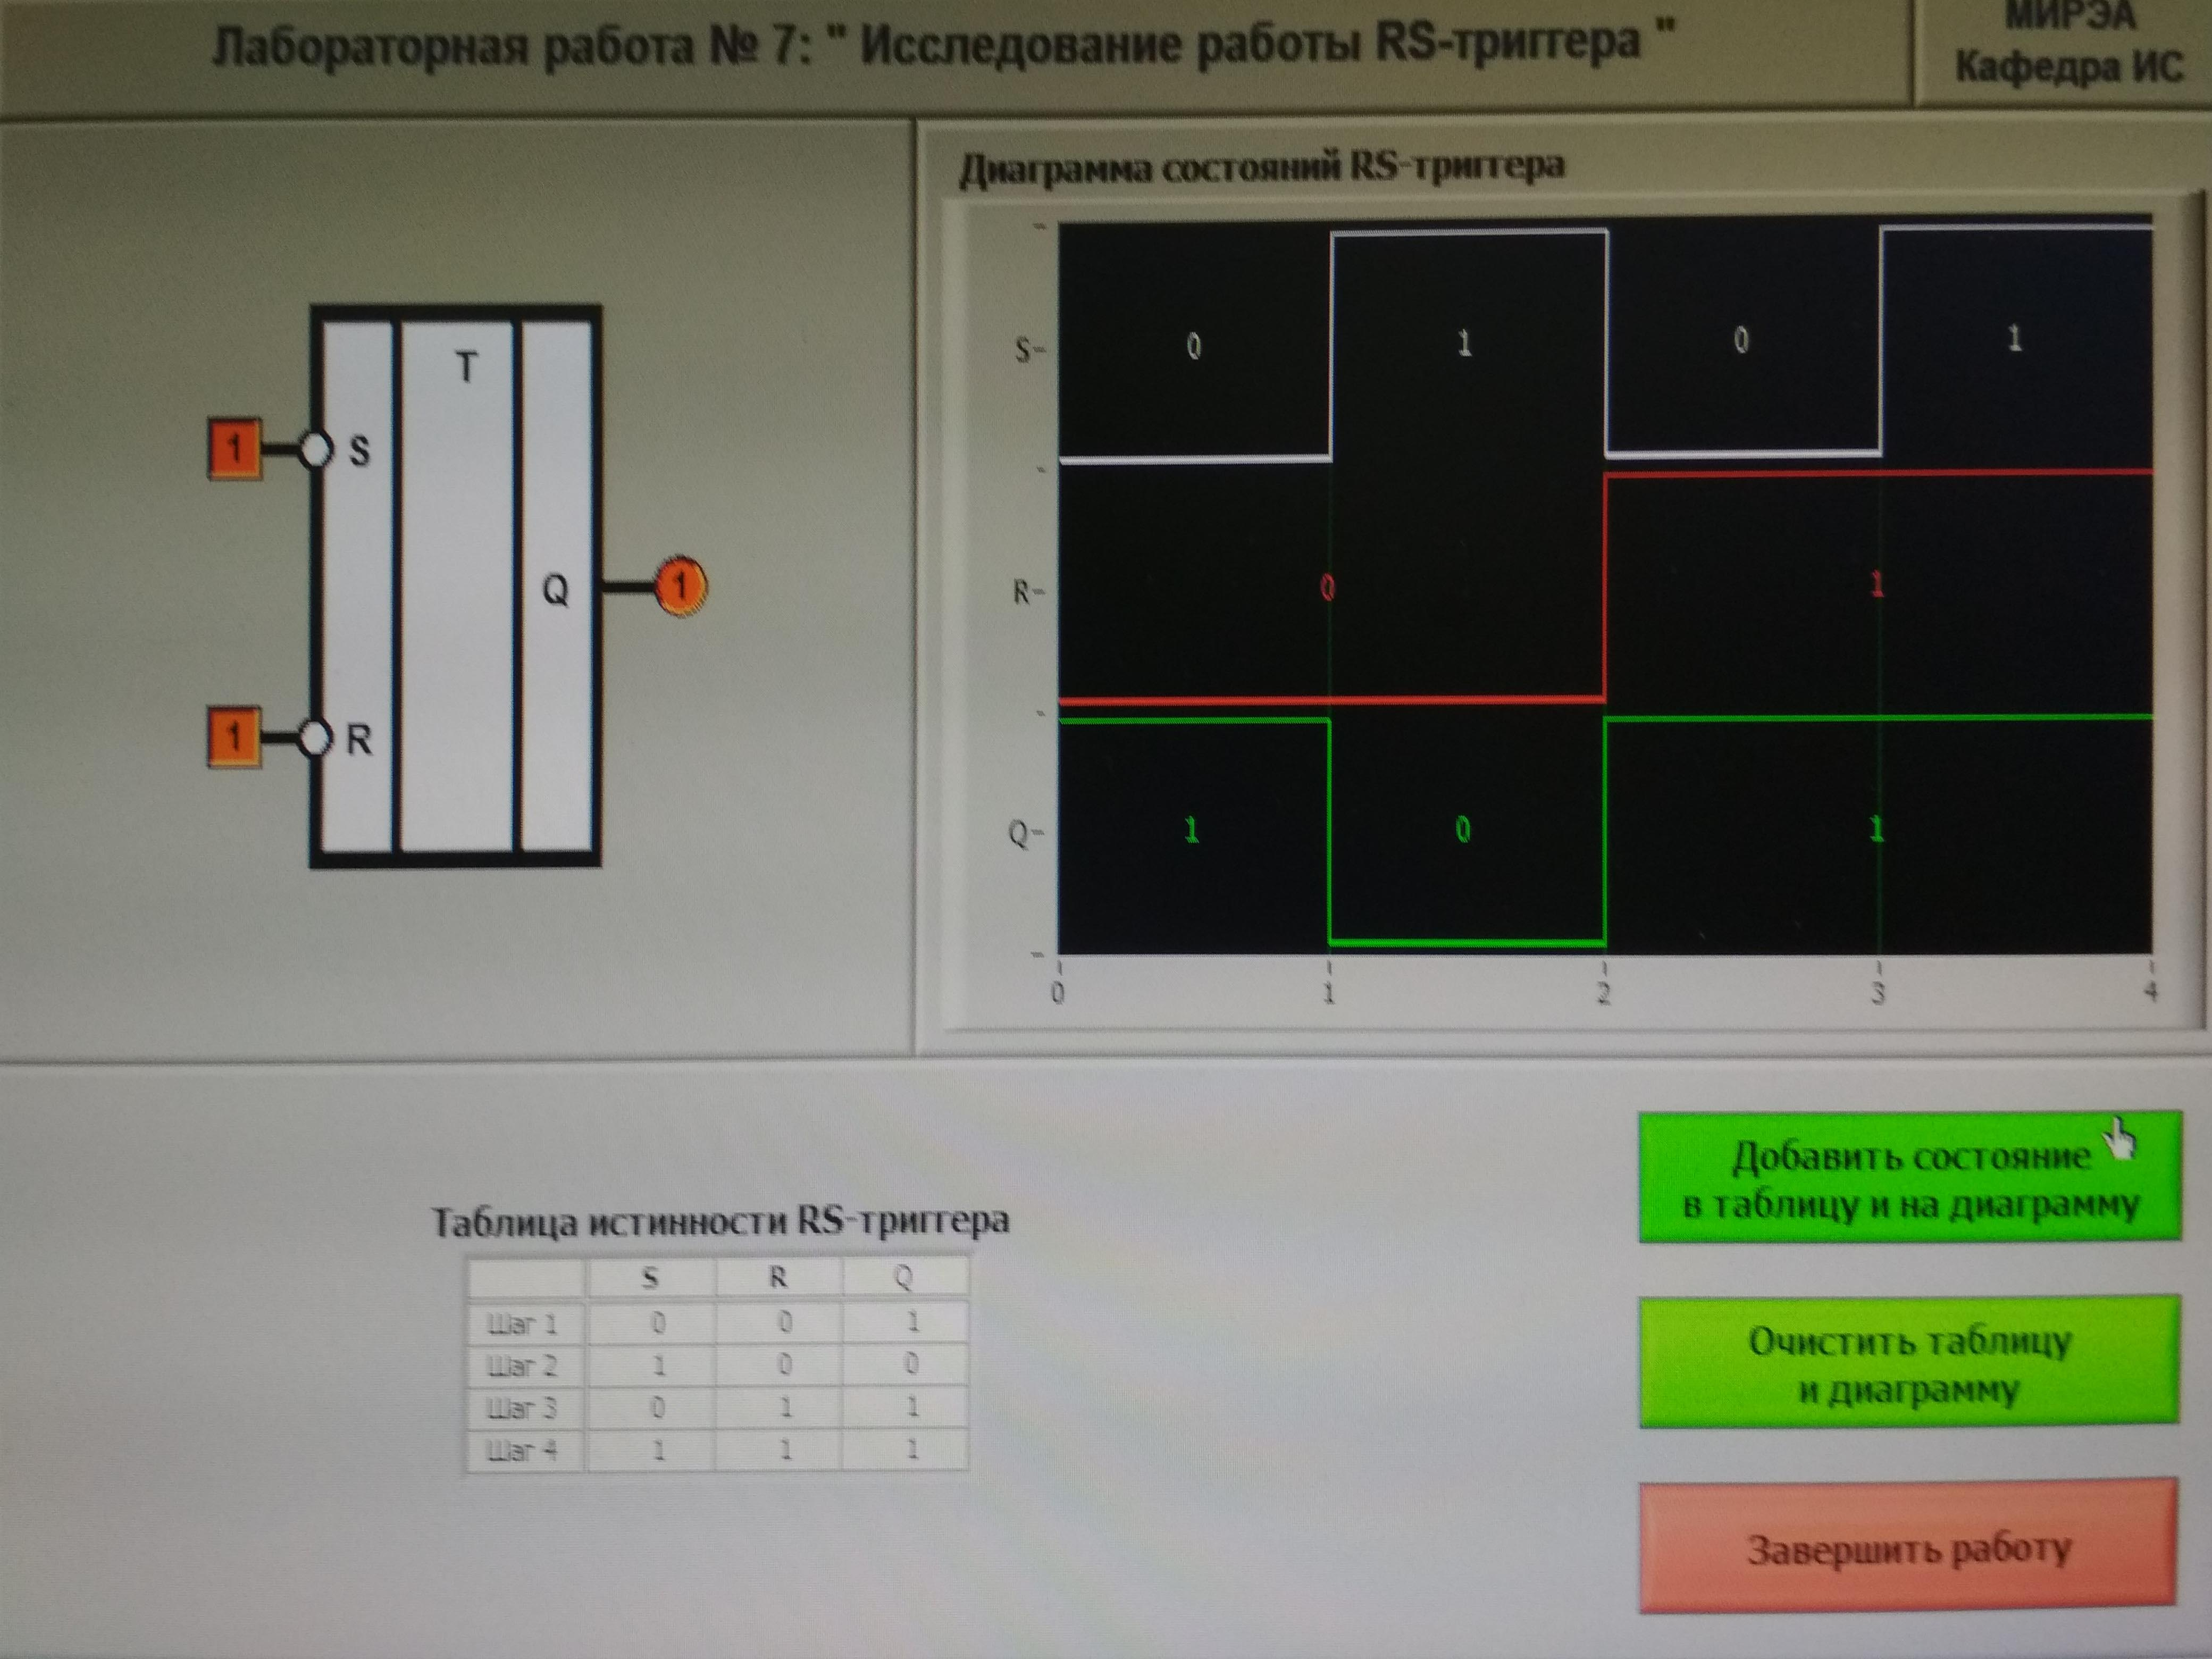
\includegraphics[width=0.95\linewidth]{imgs/7/1}
	\caption{Результат работы RS триггера}
	\label{fig:7_}
\end{figure}

% Нет ли ошибок в самом задании?
\begin{table}[H]
	\centering
	\caption{Переключение состояния RS-триггера}
	\label{tab:lab_07}
	\begin{tabular}{|c|c|c|c|}
		\hline
		Выход $Q_n$ & Вход R   & Вход S   & Выход $Q_{n+1}$ \\ \hline
		0           & $\times$ & 0        &                 \\ \hline
		0           & 0        & 1        & 0               \\ \hline
		1           & 1        & 0        & 1               \\ \hline
		1           & 0        & $\times$ &                 \\ \hline
	\end{tabular}
\end{table}

При подаче сигнала R состояние триггера устанавливается в 1.
При подаче сигнала S состояние триггера устанавливается в 0.
При подаче обоих сигналов триггер хранит состояние.
Если сигнал не подан, состояние триггера не определено.

Элемент SN74LS279A - Low-Voltage BiCMOS Technology

Сочетает 4 RS триггера в одном корпусе

Характеристики:

\begin{figure}[H]
	\centering
	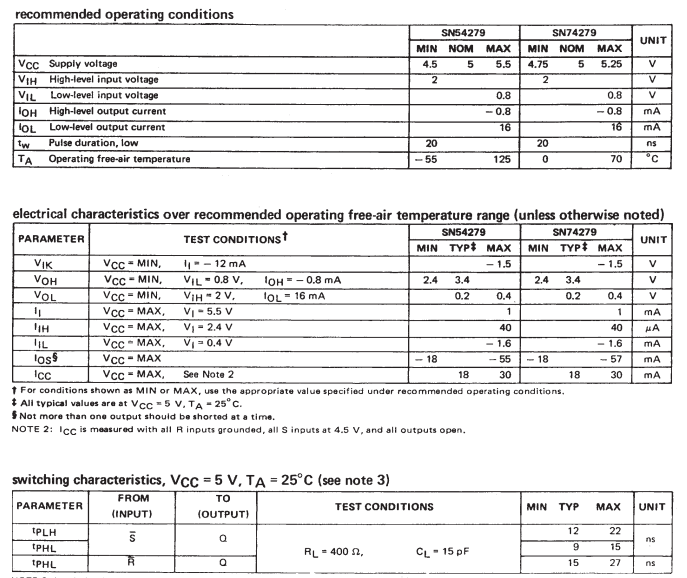
\includegraphics[width=0.95\linewidth]{imgs/7/ti}
	\caption{Парамеры триггера}
	\label{fig:7_ti}
\end{figure}

